\documentclass[11pt,a4paper]{article}
\usepackage[T1]{fontenc}
\usepackage[utf8]{inputenc}
\usepackage{lmodern,microtype}
\usepackage[margin=25mm]{geometry}
\usepackage{amsmath,amssymb,amsthm,mathtools}
\usepackage{booktabs,array,enumitem}
\usepackage{xcolor}
\usepackage{tikz}
\usetikzlibrary{arrows.meta,positioning,fit,calc,shapes.geometric}
\usepackage{pgfplots}
\pgfplotsset{compat=1.16}
\usepackage[colorlinks=true,linkcolor=blue!60!black,citecolor=teal!70!black,urlcolor=blue!60!black]{hyperref}
\setlength{\emergencystretch}{3em}
\allowdisplaybreaks[1]
\setlist{itemsep=2pt,topsep=3pt}

\newtheorem{theorem}{Theorem}[section]
\newtheorem{lemma}[theorem]{Lemma}
\newtheorem{proposition}[theorem]{Proposition}
\newtheorem{corollary}[theorem]{Corollary}
\newtheorem{conjecture}[theorem]{Conjecture}
\newtheorem{imported}[theorem]{Imported theorem}
\newtheorem*{thmA}{Theorem A (order-one drift)}
\newtheorem*{thmB}{Theorem B (unconditional Kronecker Nystr\"om)}
\newtheorem*{thmC}{Theorem C (trace estimation with real product queries)}
\newtheorem*{thmD}{Theorem D (domination of benchmark budgets)}
\newtheorem*{thmE}{Theorem E (the sharp exponent is bracketed)}
\newtheorem*{thmF}{Theorem F (other probe laws)}
\theoremstyle{definition}\newtheorem{definition}[theorem]{Definition}
\theoremstyle{remark}\newtheorem{remark}[theorem]{Remark}
\numberwithin{equation}{section}

\newcommand{\E}{\mathbb E}
\newcommand{\Prob}{\mathbb P}
\newcommand{\R}{\mathbb R}
\newcommand{\C}{\mathbb C}
\newcommand{\tr}{\operatorname{tr}}
\newcommand{\rank}{\operatorname{rank}}
\newcommand{\range}{\operatorname{range}}
\newcommand{\Var}{\operatorname{Var}}
\newcommand{\diag}{\operatorname{diag}}
\newcommand{\norm}[1]{\lVert#1\rVert}
\newcommand{\eps}{\varepsilon}
\newcommand{\Nys}{\mathcal N}
\newcommand{\opt}{\mathrm{opt}}

\title{\bfseries Product-Probe Drift,\\ Kronecker Nystr\"om Approximation, and Trace Estimation\\[4pt]
\large Residual progress from moments near order one}
\author{}
\date{29 September 2026}

% Shared manuscript typography. Keep this file beside the manuscript folders.
\usepackage{needspace}
\usepackage{etoolbox}
\linespread{1.08}
\setlength{\parskip}{0.38em plus 0.08em minus 0.05em}
\setlength{\parindent}{1.25em}
\setlength{\emergencystretch}{2em}
\setlist{itemsep=4pt,topsep=6pt,parsep=2pt}
\renewcommand{\arraystretch}{1.16}
\setlength{\tabcolsep}{6pt}
\AtBeginDocument{%
  \setlength{\abovedisplayskip}{10pt plus 2pt minus 2pt}%
  \setlength{\belowdisplayskip}{10pt plus 2pt minus 2pt}%
  \setlength{\abovedisplayshortskip}{5pt plus 2pt}%
  \setlength{\belowdisplayshortskip}{8pt plus 2pt minus 2pt}%
}
\makeatletter
\def\th@plain{%
  \thm@preskip=10pt plus 2pt minus 2pt
  \thm@postskip=10pt plus 2pt minus 2pt
  \itshape
}
\def\th@definition{%
  \thm@preskip=10pt plus 2pt minus 2pt
  \thm@postskip=10pt plus 2pt minus 2pt
  \normalfont
}
\def\th@remark{%
  \thm@headfont{\itshape}%
  \thm@preskip=9pt plus 2pt minus 2pt
  \thm@postskip=9pt plus 2pt minus 2pt
  \normalfont
}
\makeatother
\AtBeginEnvironment{proof}{\Needspace{4\baselineskip}}
\widowpenalty=10000
\clubpenalty=10000
\displaywidowpenalty=10000
\raggedbottom


\begin{document}
\maketitle

\begin{abstract}
A product probe can make useful progress without embedding a prescribed
subspace. We prove that one fresh spherical or Gaussian tensor probe reduces
the trace of every positive-semidefinite residual \(R\) by at least
\(\tr(R^2)/(\kappa\tr R)\) in expectation. The constant \(\kappa\) is the
exponential of a directional moment slope at order one, improving the
usual fourth-moment constant in every tensor factor. This gives Nystr\"om
error bounds for arbitrary eigenvectors, including a relative trace-tail
guarantee and Schatten-norm decay. Combined with Holden's diagonal-control
estimator, it yields a nonadaptive real product-query bound of order
\((N\kappa/\varepsilon^2)^{1/3}\), with \(q+1\) calls per complex probe.
A spike-plus-flat example brackets the optimal drift exponent between a
Chernoff rate and the order-one slope. We also give independent-factor,
fresh-row, and CountSketch-block versions, while leaving the unrestricted
minimax trace-query complexity open.
\end{abstract}

\tableofcontents

%======================================================================
\section{Introduction and main results}\label{sec:intro}
%======================================================================

\subsection{The query model}
A query to an unknown real symmetric matrix $A\succeq0$ must be a rank-one
tensor:
\begin{equation}\label{eq:oracle}
 (x_1,\ldots,x_q)\longmapsto A(x_1\otimes\cdots\otimes x_q),
 \qquad x_j\in\R^{n_j},\quad N=\textstyle\prod_jn_j .
\end{equation}
The oracle returns the entire vector. We count oracle calls; exact arithmetic
and storage are not charged. For trace estimation the goal is to output
$\widehat T$ with $|\widehat T-\tr A|\le\eps\tr A$ with probability at least
$2/3$, for every fixed input, and we then take $n_j=n$, $N=n^q$,
$0<\eps<1/2$. Meyer, Swartworth and Woodruff formulated Kronecker
matrix--vector complexity and list tight Kronecker trace estimation as open
\cite{MSW}; the catalogue problem RA-11 asks for the joint dependence on
$(n,q,\eps)$ \cite{RA11cat}. Meyer and Avron showed that Hutchinson-type
averaging is exponentially bad in $q$ \cite{MA}.

A full response $Az$ can do more than a scalar $z^*Az$: it can build a PSD
Nystr\"om approximation $\widehat A$ whose trace is known exactly, after which
only the residual trace must be estimated. The benefit depends on how much
residual mass each legal probe removes. This \emph{progress}, rather than an
embedding of a prescribed subspace, is the central object of the paper.

\subsection{Probe laws and the order-one constant}
A \emph{real probe} is $z=x_1\otimes\cdots\otimes x_q$ with $x_j$ independent
and uniform on the real sphere of radius $\sqrt{n_j}$. A \emph{complex probe}
uses the complex spheres of the same radii; for a real matrix it supplies the
real two-column block $W=[\Re z\ \Im z]$, whose columns are dependent and are
always analyzed together. For a real probe put $W=z$. Gaussian factors give
exactly the same Nystr\"om outputs (Section~\ref{sec:geometry}), so real
probes are the columns of a Gaussian Khatri--Rao sketch. Define
\begin{align}
 D_n^{\R}&=\log n+\psi(3/2)-\psi(n/2+1),&
 \kappa_{\R}&=\exp\Bigl(\sum_{j=1}^qD_{n_j}^{\R}\Bigr),\label{eq:kreal}\\
 D_n^{\C}&=\log n+1-H_n,&
 \kappa_{\C}&=\exp\Bigl(\sum_{j=1}^qD_{n_j}^{\C}\Bigr),\label{eq:kcomplex}
\end{align}
with $\psi=(\log\Gamma)'$ and $H_n=\sum_{a\le n}a^{-1}$. Write $\kappa$ for the
constant of the chosen law. For $n=2$, $e^{D_2^{\R}}=e/2=1.35914$ and
$e^{D_2^{\C}}=2/\sqrt e=1.21306$, against fourth-moment constants $3/2$ and $4/3$.

For a sketch $Z$ put $\Nys_A(Z)=AZ(Z^{\mathsf T}AZ)^\dagger Z^{\mathsf T}A$, let
$\widehat A_m$ be the Nystr\"om approximation built from $m$ independent probes
(or blocks), $R_m=A-\widehat A_m$, $T=\tr A$ and
$\tau_r=\tau_r(A)=\sum_{i>r}\lambda_i(A)$.

\subsection{Main results}

\begin{thmA}[Theorem~\ref{thm:drift}]
For every fixed nonzero real $R\succeq0$ and one fresh probe or block $W$,
with $R'=R-RW(W^{\mathsf T}RW)^\dagger W^{\mathsf T}R$,
\[
 0\preceq R'\preceq R,\qquad
 \E(\tr R-\tr R')\ \ge\ \frac{\tr(R^2)}{\kappa\,\tr R}.
\]
More generally, for independent isotropic factor laws with directional moment
functions $m_j(p)$, the same holds with
$\kappa=\lim_{\beta\downarrow0}\prod_jm_j(1+\beta)^{1/\beta}$.
\end{thmA}

\begin{thmB}[Theorems~\ref{thm:relative}, \ref{thm:schatten}, \ref{thm:op}]
For every real PSD input \(A\), with no hypothesis on its eigenvectors:
\begin{enumerate}[label=(\roman*)]
\item The Frobenius residual satisfies
\[
 \E\|A-\widehat A_m\|_F^2
 \le\frac{\kappa T^2}{m+\kappa T^2/\|A\|_F^2}
 \le\frac{\kappa T^2}{m}.
\]
\item Let \(1\le r<\rank A\) and \(0<\eps\le1\).
The budget
\[
 m\ge\left\lceil\kappa r\left[
 \eps^{-1}+\log(\eps^{-1})+\log(T/\tau_r)
 \right]\right\rceil
\]
ensures \(\E\tr(A-\widehat A_m)\le(1+\eps)\tau_r\).
This concerns the full, untruncated approximation.
\item For every \(p>1\),
\[
 \E\tr R_m^p
 \le T^p\left(1+\frac{m}{\kappa(p-1)}\right)^{-(p-1)}.
\]
\item For \(0<\mu\le T\),
\[
 \Prob\{\|R_m\|\ge\mu\}
 \le\min\left\{1,\frac{2T}{\mu}
           e^{-m\mu/(2\kappa T)}\right\}.
\]
In particular, \(m\ge(2\kappa T/\rho)\log(2T/(\rho\delta))\)
makes \(\widehat A_m+\rho I\) a factor-two preconditioner for
\(A+\rho I\), with probability at least \(1-\delta\), when \(0<\rho\le T\).
\end{enumerate}
\end{thmB}

\begin{thmC}[Theorem~\ref{thm:queries}]
Choose one of the two pairs
\[
 (b,\kappa)=(1,e^{qD_n^{\R}})
 \quad\text{or}\quad
 (b,\kappa)=(q+1,e^{qD_n^{\C}}).
\]
There is a nonadaptive unbiased estimator using \(bm+2s\) real product
queries with
\[
 \Var\widehat T\le\frac{2N\kappa T^2}{ms^2}.
\]
Set \(L_b=(6bN\kappa/\eps^2)^{1/3}\). At success probability \(2/3\),
the query budget is
\[
 \mathcal D_b=\min\{N,\ b\lceil L_b/b\rceil+2\lceil L_b\rceil\}
 \le\min\{N,3L_b+b+2\}.
\]
We take the smaller of the real and complex budgets.
For \(n=2\), the real branch has the smaller leading term exactly when
\(q\le30\). In the complex implementation, retaining the \(q+1\)
interpolation vectors is pathwise at least as accurate as keeping only
the two-column block.
\end{thmC}

\begin{thmD}[Theorem~\ref{thm:domination}]
The rounded drift budget is at most either benchmark budget defined
in Section~\ref{sec:comparison}, for every admissible \((n,q,\eps)\).
Before the exact basis cap, their leading terms exceed the drift
leading term by factors of at least \(18.44\) and \(44.23\), respectively.
For complex binary factors, the optimized fractional benchmark also
has an \(\exp(\Theta(\sqrt q))\) coefficient overhead
(Proposition~\ref{prop:overhead}); the drift bound has a polynomial
prefactor at \(\eps=(9/10)^q\).
\end{thmD}

\begin{thmE}[Theorem~\ref{thm:bracket}]
Let $\kappa_\opt(n,q)$ be the best constant in the drift inequality of
Theorem~A for the real one-column law or the complex block law, and
$\gamma_n=-\min_{0\le\lambda\le1}\log c_n(\lambda)$, where $c_n$ is the local
moment function of the same field. If $n^q\ge4$ then
\[
 \tfrac1{32}\,e^{q\gamma_n}\ \le\ \kappa_\opt(n,q)\ \le\ e^{qD_n}.
\]
For $n=2$ complex, $\gamma_2=\log2-1-\log\log2=0.059660$ and $D_2^{\C}=0.193147$;
for $n=2$ real, $[\gamma_2^{\R},D_2^{\R}]=[0.109117,0.306853]$.
\end{thmE}

If the lower end is the truth (Conjecture~\ref{conj:gamma}), the binary running
base drops from $1.441482$ to $1.378748$; the benchmark obtained by this analysis with a subexponential drift
constant is $(200/81)^{1/3}=1.351600$.

\begin{thmF}[Section~\ref{sec:otherlaws}]
The progress method also gives the following sufficient constants:
\begin{enumerate}[label=(\roman*)]
\item Independent isotropic sub-Gaussian factors satisfying
\(\E e^{\langle x_j,u\rangle^2/K_j^2}\le2\) have
\(\kappa\le\prod_j2K_j^2(K_j^2-1)\).
\item Independent fresh SRHT rows have the dimension-uniform bound
\(\kappa_0=e^{2-\gamma}/2=2.074328\), where \(\gamma\) is Euler's constant.
\item A fresh \(b\)-row CountSketch block has
\(\kappa_b=1+2/b\), counting the whole block as one update.
\end{enumerate}
The fresh-row guarantee requires independent sign redraws.
The block bound can lose a factor of order \(b\) on a flat residual.
\end{thmF}

\clearpage
\subsection{Roadmap}

\begin{figure}[ht]
\centering
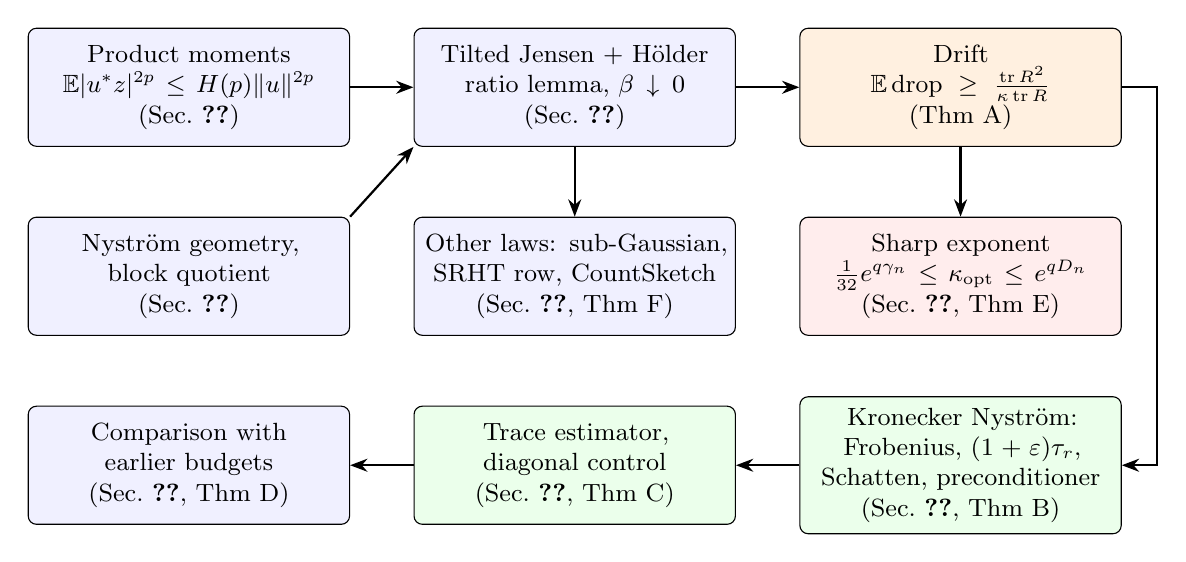
\begin{tikzpicture}[
  box/.style={draw,rounded corners=3pt,align=center,font=\small,inner sep=4pt,
     text width=38mm,minimum height=15mm,fill=#1},
  box/.default=blue!6,
  arr/.style={-{Stealth[length=2.2mm]},thick}]
\node[box] (mom) at (0,0) {Product moments\\ $\E|u^*z|^{2p}\le H(p)\norm u^{2p}$\\ (Sec.~\ref{sec:moments})};
\node[box] (ratio) at (4.9,0) {Tilted Jensen + H\"older\\ ratio lemma, $\beta\downarrow0$\\ (Sec.~\ref{sec:drift})};
\node[box=orange!12] (drift) at (9.8,0) {Drift\\ $\E\,\mathrm{drop}\ge\frac{\tr R^2}{\kappa\tr R}$\\ (Thm A)};
\node[box] (geo) at (0,-2.4) {Nystr\"om geometry,\\ block quotient\\ (Sec.~\ref{sec:geometry})};
\node[box] (other) at (4.9,-2.4) {Other laws: sub-Gaussian,\\ SRHT row, CountSketch\\ (Sec.~\ref{sec:otherlaws}, Thm F)};
\node[box=red!7] (sharp) at (9.8,-2.4) {Sharp exponent\\ $\frac{1}{32}e^{q\gamma_n}\le\kappa_\opt\le e^{qD_n}$\\ (Sec.~\ref{sec:sharp}, Thm E)};
\node[box=green!8] (nys) at (9.8,-4.8) {Kronecker Nystr\"om:\\ Frobenius, $(1+\eps)\tau_r$,\\ Schatten, preconditioner\\ (Sec.~\ref{sec:consequences}, Thm B)};
\node[box=green!8] (trace) at (4.9,-4.8) {Trace estimator,\\ diagonal control\\ (Sec.~\ref{sec:estimator}, Thm C)};
\node[box] (comp) at (0,-4.8) {Comparison with\\ earlier budgets\\ (Sec.~\ref{sec:comparison}, Thm D)};
\draw[arr] (mom) -- (ratio);
\draw[arr] (ratio) -- (drift);
\draw[arr] (geo.north east) -- (ratio.south west);
\draw[arr] (ratio) -- (other);
\draw[arr] (drift) -- (sharp);
\draw[arr] (drift.east) -- ++(0.45,0) |- (nys.east);
\draw[arr] (nys) -- (trace);
\draw[arr] (trace) -- (comp);
\end{tikzpicture}
\caption{Logical structure of the paper.}
\label{fig:roadmap}
\end{figure}



\subsection{Prior work and the contribution}
The full-vector Kronecker oracle and its distinction from scalar
quadratic-form access are due to Meyer--Swartworth--Woodruff \cite{MSW}.
Meyer--Avron \cite{MA} analyze product-probe Hutchinson estimators, including
the advantage of spherical and complex factors. Their estimator-specific
lower bounds do not determine the complexity of the full-vector model.

Holden's public manuscript \cite{Holden} already gives the complex
order-one constant \(D_n^{\C}\), fractional empirical-average bounds,
real interpolation of complex responses, diagonal control, and finite
angular laws. We use these constructions with explicit attribution.
Sections~\ref{sec:geometry}--\ref{sec:estimator} reproduce the arguments
needed here, so the present guarantees do not depend on a private note.

The new step proposed here is Lemma~\ref{lem:ratio}: a numerator-weighted
change of measure converts moments arbitrarily close to order one into a
uniform expected quotient bound. It yields progress for every PSD
residual, rather than an embedding guarantee for a fixed subspace.
The resulting Nystr\"om analysis uses the standard projection identity
and the residual-contraction mechanism of Chen--Epperly--Tropp--Webber
\cite{CETW}. The convex-potential and ramp arguments adapt
Epperly \cite[Lemma~4.2]{Epperly}; they are not claimed as new matrix
inequalities. Divan--Gilles \cite{DG} give recent convergence results for
randomized and approximate pivoting in a different sampling model.

Cama\~no--Epperly--Meyer--Tropp \cite{CEMT} obtain structured Nystr\"om
guarantees through oblivious subspace injections. Saibaba--Verma--Ballard
\cite{SVB} and Beretta--Musco \cite{BM} develop Khatri--Rao low-rank and
subspace-embedding analyses. Our contribution is the explicit
order-one progress bound, its application to untruncated approximation
and trace estimation, and the spike-plus-flat exponent bracket.
These are comparisons of proof mechanisms and guarantees; no sharp
OSE result or complete resolution of RA-11 is asserted. The literature
search is current to 29 September 2026 and does not certify priority.

\paragraph{Notation and scope.}
We use \(\|\cdot\|\) for the Euclidean norm on vectors and the operator
norm on matrices; \(\|\cdot\|_F\) is the Frobenius norm.
Eigenvalues of a PSD matrix are ordered decreasingly, and
\(M^\dagger\) denotes the Moore--Penrose pseudoinverse. Expectations
are over the probes, with the input matrix fixed. All oracle and
interpolation statements use exact arithmetic. The bounds count calls,
not storage or arithmetic work.

%======================================================================
\section{Nystr\"om geometry and sequential updates}\label{sec:geometry}
%======================================================================
If $P_Z$ is the orthogonal projector onto $\range(A^{1/2}Z)$, then
\begin{equation}\label{eq:projector}
 \Nys_A(Z)=A^{1/2}P_ZA^{1/2},
\end{equation}
since $B(B^{\mathsf T}B)^\dagger B^{\mathsf T}$ is the range projector of $B=A^{1/2}Z$.
Thus $0\preceq\Nys_A(Z)\preceq A$, and $\Nys_A(Z)$ is monotone in $\range Z$:
if $\range Z\subseteq\range Z'$ then $A-\Nys_A(Z')\preceq A-\Nys_A(Z)$.

\begin{lemma}[Adding a block]\label{lem:sequential}
Let $R=A-\Nys_A(Z)$ and let $W$ be an additional real block. Then
\begin{equation}\label{eq:sequential}
 A-\Nys_A([Z\ W])=R-RW(W^{\mathsf T}RW)^\dagger W^{\mathsf T}R .
\end{equation}
\end{lemma}
\begin{proof}
Write \(P=P_Z\) and orthogonalize the new block against the old sketch:
\[
 H=(I-P)A^{1/2}W.
\]
The enlarged sketch range is the orthogonal sum of
\(\range(A^{1/2}Z)\) and \(\range H\). Its projector is therefore
\[
 P_{[Z\ W]}=P+H(H^{\mathsf T}H)^\dagger H^{\mathsf T}.
\]
The two identities
\[
 H^{\mathsf T}H=W^{\mathsf T}RW,
 \qquad A^{1/2}H=RW
\]
now turn the projector formula \eqref{eq:projector} into
\eqref{eq:sequential}.
\end{proof}

Independently drawn blocks can therefore be analyzed as successive updates,
conditioning on the current residual; the algorithm never inspects the
residual before choosing its queries.

\begin{lemma}[Scalar lower bound for block progress]\label{lem:block}
For complex $z$ and $W=[\Re z\ \Im z]$, and real $R\succeq0$, the trace drop in
\eqref{eq:sequential} is at least
\begin{equation}\label{eq:quotient}
 \frac{z^*R^2z}{z^*Rz},
\end{equation}
with the convention $0/0=0$. For a real one-column probe the drop equals this quotient.
\end{lemma}
\begin{proof}
Let $P$ project onto $\range(R^{1/2}W)$; the drop is $\tr(PR)$. If $z^*Rz>0$,
the complex unit vector $v=R^{1/2}z/\sqrt{z^*Rz}$ lies in the complexification of
this real range, so $P-vv^*\succeq0$ and $\tr(PR)\ge v^*Rv$, which is
\eqref{eq:quotient}. If $z^*Rz=0$ both columns are annihilated by $R^{1/2}$.
\end{proof}

\paragraph{Gaussian factors.}
A standard Gaussian vector is a positive radius times an independent uniform
direction, and multiplying a sketch column (or a whole complex block) by a
nonzero scalar leaves \eqref{eq:projector} unchanged. Hence Gaussian
Khatri--Rao columns have exactly the same Nystr\"om output, under this
coupling, as spherical product columns; every result below applies to them.
With continuous factors, rank-$s$ inputs are recovered after $s$ probes almost
surely: product vectors span the space, so a suitable minor is a nonzero
polynomial in the factor coordinates.

%======================================================================
\section{Product moments and the constant at order one}\label{sec:moments}
%======================================================================
The probe is isotropic, $\E zz^*=I$. For $p>-1/2$ (real) or $p>-1$ (complex) put
\begin{align}
 c_n^{\R}(p)&=\frac{n^p\Gamma(p+1/2)\Gamma(n/2)}{\Gamma(1/2)\Gamma(n/2+p)},&
 c_n^{\C}(p)&=\frac{n^p\Gamma(p+1)\Gamma(n)}{\Gamma(n+p)},\label{eq:cn}
\end{align}
and $H(p)=\prod_jc_{n_j}(p)$, the superscript matching the probe field.
For $n=2$: $c_2^{\C}(p)=2^p/(1+p)$.

\begin{lemma}[Directional and quadratic moments]\label{lem:moments}
Let the factors $x_j$ be independent and isotropic, and suppose
$\E|u^*x_j|^{2p}\le m_j(p)\norm u^{2p}$ for all $u$, with $p\ge1$. Then for
every $u$ and every Hermitian $B\succeq0$,
\begin{equation}\label{eq:tensor-moments}
 \E|u^*z|^{2p}\le M(p)\norm u^{2p},\qquad \E(z^*Bz)^p\le M(p)(\tr B)^p,
 \qquad M(p)=\prod_jm_j(p).
\end{equation}
For spherical factors one may take $m_j=c_{n_j}$, with equality in the
directional bound for a single factor, so $M=H$.
\end{lemma}
\begin{proof}
For one spherical factor and unit $u$, rotational invariance reduces
$|u^*x|^2$ to $n$ times the squared first coordinate of a uniform unit vector,
which is $\mathrm{Beta}(1/2,(n-1)/2)$ (real) or $\mathrm{Beta}(1,n-1)$ (complex);
the beta moments give \eqref{eq:cn}. For $n=1$ both equal one.

To tensorize, decompose $u=\sum_au_a\otimes e_a$ in the last factor. Conditioning on
$z_{<q}=x_1\otimes\cdots\otimes x_{q-1}$, the vector $v_a=u_a^*z_{<q}$ is fixed and
$u^*z=\sum_a v_a(x_q)_a$, so the local bound leaves
$m_q(p)(\sum_a|u_a^*z_{<q}|^2)^p$. Minkowski in $L^p$ gives
\[
 \Bigl\|\sum_a|u_a^*z_{<q}|^2\Bigr\|_{L^p}
 \le\sum_a\bigl(\E|u_a^*z_{<q}|^{2p}\bigr)^{1/p}
 \le\Bigl(\prod_{j<q}m_j(p)\Bigr)^{1/p}\sum_a\norm{u_a}^2,
\]
and induction proves the directional bound. For the quadratic bound write
$B=\sum_ib_iu_iu_i^*$ with unit $u_i$ and apply Minkowski:
$\norm{z^*Bz}_{L^p}\le\sum_ib_i\norm{|u_i^*z|^2}_{L^p}\le M(p)^{1/p}\tr B$.
\end{proof}

\begin{lemma}[The order-one constant]\label{lem:slope}
Each $p\mapsto\log m(p)$ that is a supremum of logarithmic moments
$\log\E|u^*x|^{2p}$ over unit $u$ is convex, with $m(1)=1$ under isotropy.
Consequently $\beta\mapsto M(1+\beta)^{1/\beta}$ is nondecreasing on $(0,\infty)$ and
\[
 \kappa:=\lim_{\beta\downarrow0}M(1+\beta)^{1/\beta}=\inf_{\beta>0}M(1+\beta)^{1/\beta}\le M(2).
\]
For spherical factors $\kappa=\kappa_{\R}$ or $\kappa_{\C}$ of
\eqref{eq:kreal}--\eqref{eq:kcomplex}, and $D_n<\log c_n(2)$ for $n\ge2$.
\end{lemma}
\begin{proof}
$p\mapsto\log\E X^p$ is convex by H\"older, and a supremum of convex functions
is convex. A convex function vanishing at $0$ has nondecreasing secant slopes
$\beta\mapsto\log M(1+\beta)/\beta$, whose limit at $0$ is the right derivative.
For spheres, differentiate \eqref{eq:cn} at $p=1$: in the complex case
$\log n+\psi(2)-\psi(n+1)=\log n+1-H_n$ using $\psi(k+1)=H_k-\gamma$; in the
real case $\log n+\psi(3/2)-\psi(n/2+1)$. Strict convexity for $n\ge2$ gives
$D_n<\log c_n(2)-\log c_n(1)$.
\end{proof}

Since $\E X=1$ for $X=|u^*x|^2$ with unit $u$, the slope is $\E[X\log X]\ge0$: $\log\kappa$
is a sum of size-biased logarithmic moments, and $\kappa\ge1$.

\begin{center}
\renewcommand{\arraystretch}{1.15}
\begin{tabular}{@{}lll@{}}
\toprule
Local law & Order-one constant $e^{D_n}$ & Fourth moment $c_n(2)$\\
\midrule
Real, $n=2$ & $e/2=1.359141$ & $3/2$\\
Complex, $n=2$ & $2/\sqrt e=1.213061$ & $4/3$\\
Real, general $n$ & $e^{\log n+\psi(3/2)-\psi(n/2+1)}\ \uparrow\ e^{2-\gamma}/2$ & $3n/(n+2)$\\
Complex, general $n$ & $e^{\log n+1-H_n}\ \uparrow\ e^{1-\gamma}$ & $2n/(n+1)$\\
\bottomrule
\end{tabular}
\end{center}
Improving each factor gives an exponential improvement in $q$.

%======================================================================
\section{From fractional moments to expected progress}\label{sec:drift}
%======================================================================
The numerator and denominator of \eqref{eq:quotient} depend on the same probe.
A change of measure by the numerator keeps this dependence and reduces the
problem to a mixed moment.

\begin{lemma}[Mixed moment and ratio conversion]\label{lem:ratio}
Let $z$ be isotropic and satisfy the directional bound of
\eqref{eq:tensor-moments} at $p=1+\beta$, $\beta>0$. For nonzero PSD $B,R$ with
$\ker R\subseteq\ker B$,
\begin{equation}\label{eq:ratio-bound}
 \E\frac{z^*Bz}{z^*Rz}\ \ge\ \frac{\tr B}{M(1+\beta)^{1/\beta}\tr R}.
\end{equation}
\end{lemma}
\begin{proof}
Set \(a=z^*Bz\), \(b=z^*Rz\), and \(p=1+\beta\).
The kernel condition ensures \(a=0\) on \(\{b=0\}\), and isotropy gives
\(\E a=\tr B\).

\emph{Step 1: weight by the numerator.}
Define the probability measure
\[
 dQ=\frac{a}{\tr B}\,dP.
\]
Under \(Q\), the denominator is positive almost surely. Jensen's
inequality for \(t\mapsto t^{-1/\beta}\) gives
\begin{equation}\label{eq:tilted}
 \E\frac ab
 =\tr B\,\E_Q b^{-1}
 \ge \tr B\,(\E_Q b^\beta)^{-1/\beta}.
\end{equation}
The conclusion also holds when the left side is infinite.

\emph{Step 2: bound the mixed moment.}
Take a spectral decomposition \(B=\sum_i b_i u_i u_i^*\) with unit
eigenvectors. H\"older with conjugate exponents \(p\) and \(p/\beta\),
followed by Lemma~\ref{lem:moments}, yields
\begin{align*}
 \E[|u_i^*z|^2 b^\beta]
 &\le (\E|u_i^*z|^{2p})^{1/p}
       (\E b^p)^{\beta/p}\\
 &\le M(p)^{1/p}M(p)^{\beta/p}(\tr R)^\beta\\
 &=M(p)(\tr R)^\beta.
\end{align*}
Summing with weights \(b_i\), we obtain
\[
 \E_Q b^\beta
 =\frac{\E[a b^\beta]}{\tr B}
 \le M(p)(\tr R)^\beta.
\]
Substitution into \eqref{eq:tilted} proves \eqref{eq:ratio-bound}.
\end{proof}

\begin{theorem}[Order-one drift]\label{thm:drift}
Under the hypotheses of Lemma~\ref{lem:moments} for all $p\in(1,1+\beta_0)$, and
with $\kappa$ as in Lemma~\ref{lem:slope}, one fresh probe or complex block satisfies
$0\preceq R'\preceq R$ and
\begin{equation}\label{eq:main-drift}
 \E(\tr R-\tr R')\ge\frac{\tr(R^2)}{\kappa\tr R}.
\end{equation}
More generally, for $B\succeq0$ with $\ker R\subseteq\ker B$,
\begin{equation}\label{eq:weighted}
 \E\frac{z^*Bz}{z^*Rz}\ge\frac{\tr B}{\kappa\tr R}.
\end{equation}
\end{theorem}
\begin{proof}
Take $B=R^2$ in Lemma~\ref{lem:ratio}, bound the drop below by the quotient
(Lemma~\ref{lem:block}), and let $\beta\downarrow0$; the left side does not depend
on $\beta$. The projector representation gives $0\preceq R'\preceq R$.
\end{proof}

No lower spectral edge of a sample Gram matrix and no inverse moment are needed.
Taking $\beta=1$ gives the fourth-moment constant $M(2)$; letting $\beta\to0$
improves it without changing the algorithm.

%======================================================================
\section{Unconditional Kronecker Nystr\"om approximation}\label{sec:consequences}
%======================================================================
Let $R_t=A-\widehat A_t$ after $t$ independent probes or blocks and $T=\tr A$.
If $T=0$ then $A=0$ and everything is trivial; otherwise $R_t$ decreases in
PSD order and $\tr R_t\le T$. All statements in this section hold for every
fixed real PSD $A$, whatever its eigenvectors, and for any probe law satisfying
Theorem~\ref{thm:drift} (in particular Gaussian Khatri--Rao columns with
$\kappa=\kappa_{\R}$).

\subsection{Frobenius residual}
\begin{proposition}\label{prop:frob}
$\E\tr(R_m^2)\le\kappa T^2/m$ for every $m\ge1$.
\end{proposition}
\begin{proof}
Conditional drift gives $\E[\tr R_t-\tr R_{t+1}\mid R_t]\ge\tr(R_t^2)/(\kappa T)$.
Summing from $t=0$ to $m-1$ telescopes to $\sum_{t<m}\E\tr(R_t^2)\le\kappa T^2$.
If $0\preceq S\preceq R$ then $\tr R^2-\tr S^2=\tr((R-S)(R+S))\ge0$, so the
summands decrease and the sum is at least $m\E\tr(R_m^2)$.
\end{proof}
Section~\ref{sec:convex} sharpens this to $\kappa T^2/(m+\kappa T^2/\norm A_F^2)$.

\subsection{The \texorpdfstring{$(1+\eps)$}{(1+eps)} trace-tail theorem}
\begin{theorem}[Unconditional Kronecker Nystr\"om, relative trace error]\label{thm:relative}
Let $1\le r<\rank A$, $\tau=\tau_r(A)>0$ and $0<\eps\le1$. If
\begin{equation}\label{eq:relative-budget}
 m\ge\Bigl\lceil\kappa r\Bigl[\frac1\eps+\log\frac1\eps+\log\frac T\tau\Bigr]\Bigr\rceil,
\end{equation}
then $\E\tr R_m\le(1+\eps)\tau$. The approximation is not truncated to rank $r$.
\end{theorem}
\begin{proof}
\emph{Step 1: reduce the spectrum to the residual trace.}
Since \(R_t\preceq A\), its rank-\(r\) tail is at most \(\tau\).
The first \(r\) eigenvalues therefore sum to at least
\((\tr R_t-\tau)_+\). Cauchy--Schwarz implies
\[
 \tr R_t^2\ge\frac{(\tr R_t-\tau)_+^2}{r}.
\]
The function \(g(x)=(x-\tau)_+^2/x\), extended by \(g(0)=0\), is convex.
Above \(\tau\), it equals \(x-2\tau+\tau^2/x\); at \(\tau\) its derivative
matches the zero derivative on the interval below.

\emph{Step 2: obtain a scalar recurrence.}
Let \(f_t=\E\tr R_t\). Conditional drift and Jensen give
\begin{equation}\label{eq:cooling}
 f_{t+1}\le f_t-\frac{(f_t-\tau)_+^2}{\kappa r f_t},
\end{equation}
where a zero denominator is interpreted by continuity.
For \(u_t=f_t/\tau-1>0\), this becomes
\[
 u_t-u_{t+1}\ge\frac{u_t^2}{\kappa r(1+u_t)}.
\]

\emph{Step 3: count the steps until the target is reached.}
The decreasing convex function
\[
 F(u)=u^{-1}-\log u,
 \qquad F'(u)=-\frac{1+u}{u^2}
\]
satisfies, whenever \(u_{t+1}>0\),
\[
 F(u_{t+1})-F(u_t)
 \ge F'(u_t)(u_{t+1}-u_t)
 \ge\frac1{\kappa r}.
\]
If \(u_s>\eps\) for all \(0\le s\le t\), telescoping gives
\[
 F(u_t)\ge F(u_0)+\frac{t}{\kappa r}
 \ge-\log(T/\tau)+\frac{t}{\kappa r}.
\]
For the integer \(t\) in \eqref{eq:relative-budget}, the right side
is at least \(F(\eps)=\eps^{-1}+\log(\eps^{-1})\).
This contradicts \(u_t>\eps\), because \(F\) is decreasing.
Thus some \(s\le t\) satisfies \(f_s\le(1+\eps)\tau\), and monotonicity
of the residual trace preserves the bound at every later step.
\end{proof}

This is the scalar residual-contraction mechanism of RPCholesky analysis
\cite{CETW} with the product law charged through $\kappa$. It applies to the
full (untruncated) Nystr\"om output. For Gaussian Khatri--Rao sketches of order
$q$ with $n_j\to\infty$ the constant tends to $\kappa_0^q$, $\kappa_0=2.0743$;
e.g.\ $\kappa_0^2=4.30$ at $q=2$. Unlike results that assume a common Kronecker (Schmidt) structure of the
eigenvectors of $A$, or that rest on Gaussian equivalence, no hypothesis ties
the eigenvectors of $A$ to the tensor factors; the
price is $\kappa$ and the logarithm of $T/\tau_r$.

\subsection{Convex potentials and Schatten rates}\label{sec:convex}
\begin{theorem}[Convex-potential progress]\label{thm:convex}
Let $f:[0,\infty)\to[0,\infty)$ be finite and convex with $f(0)=0$. For nonzero
real $R\succeq0$, one fresh probe or block gives
\begin{equation}\label{eq:convex}
 \E\tr f(R')\le\tr f(R)-\frac{\tr[Rf(R)]}{\kappa\tr R}.
\end{equation}
\end{theorem}
\begin{proof}
Let \(P\) be the projector onto \(\range(R^{1/2}W)\), and set \(Q=I-P\).
The matrices \(R'=R^{1/2}QR^{1/2}\) and \(QRQ\) have the same eigenvalues,
including multiplicities of zero.

\emph{Compression.}
Choose an orthonormal eigenbasis \(v_a\) for the compression of \(R\)
to \(\range Q\). Scalar Jensen applied to the spectral measure of \(R\)
in the state \(v_a\) gives
\[
 f(v_a^*Rv_a)\le v_a^*f(R)v_a.
\]
Summing and using \(f(0)=0\), we conclude
\[
 \tr f(R')\le\tr(Qf(R))
 =\tr f(R)-\tr(Pf(R)).
\]

\emph{Expected loss of potential.}
When \(z^*Rz>0\), the unit vector
\(v=R^{1/2}z/\sqrt{z^*Rz}\) lies in the complexification of the range of \(P\).
Since \(f(R)\succeq0\),
\[
 \tr(Pf(R))\ge v^*f(R)v
 =\frac{z^*Rf(R)z}{z^*Rz}.
\]
At a zero denominator, use the zero-quotient convention.
Apply \eqref{eq:weighted} with \(B=Rf(R)\), which is PSD and vanishes
on \(\ker R\). This proves the desired bound. The compression step
is the argument of \cite[Lemma~4.2]{Epperly}.
\end{proof}

\begin{theorem}[Schatten residual decay]\label{thm:schatten}
For every real $p>1$ and $m\ge0$,
\begin{equation}\label{eq:schatten}
\begin{aligned}
 \E\tr(R_m^p)
 &\le T^p\left[
 \left(\frac{T^p}{\tr A^p}\right)^{1/(p-1)}
 +\frac m{\kappa(p-1)}
 \right]^{-(p-1)}\\
 &\le\frac{T^p}{(1+m/[\kappa(p-1)])^{p-1}}.
\end{aligned}
\end{equation}
In particular
$\E\norm{R_m}_F^2\le\kappa T^2/(m+\kappa T^2/\norm A_F^2)\le\kappa T^2/(m+\kappa)$.
\end{theorem}
\begin{proof}
\emph{Moment interpolation.}
H\"older's inequality for the eigenvalues gives
\[
 \tr R^p\le(\tr R)^{1/p}(\tr R^{p+1})^{(p-1)/p},
\]
and consequently
\[
 \tr R^{p+1}
 \ge(\tr R^p)^{p/(p-1)}(\tr R)^{-1/(p-1)}.
\]
Use \(f(x)=x^p\) in Theorem~\ref{thm:convex} and \(\tr R_t\le T\) to obtain
\[
 \E[\tr R_{t+1}^p\mid R_t]
 \le\tr R_t^p
 -\frac{(\tr R_t^p)^{p/(p-1)}}{\kappa T^{p/(p-1)}}.
\]

\emph{Solve the recurrence.}
Set \(a_t=\E\tr R_t^p/T^p\). Jensen now implies
\[
 a_{t+1}\le a_t-\kappa^{-1}a_t^{p/(p-1)}.
\]
For \(\phi(x)=x^{-1/(p-1)}\), convexity and monotonicity give, as long
as \(a_{t+1}>0\),
\[
 \phi(a_{t+1})-\phi(a_t)
 \ge\phi'(a_t)(a_{t+1}-a_t)
 \ge\frac1{\kappa(p-1)}.
\]
Summing and inverting proves the first inequality in \eqref{eq:schatten}.
If any \(a_t\) vanishes, the residual remains zero and the conclusion
is immediate. Finally \(\tr A^p\le T^p\) gives the second inequality.
\end{proof}

\subsection{Operator-norm tail and a regularized preconditioner}
\begin{theorem}[Absolute spectral error]\label{thm:op}
For $0<\mu\le T$,
\begin{equation}\label{eq:spectral}
 \Prob\{\norm{R_m}\ge\mu\}\le\min\Bigl\{1,\frac{2T}\mu\exp\Bigl(-\frac{m\mu}{2\kappa T}\Bigr)\Bigr\}.
\end{equation}
Consequently, for $0<\rho\le T$ and $0<\delta<1$, if
$m\ge(2\kappa T/\rho)\log(2T/(\rho\delta))$ then with probability at least
$1-\delta$ the matrix $P=\widehat A_m+\rho I$ satisfies
$P\preceq A+\rho I\preceq2P$, so
$\operatorname{cond}(P^{-1/2}(A+\rho I)P^{-1/2})\le2$.
\end{theorem}
\begin{proof}
Use the ramp $f(x)=(x-\mu/2)_+$, for which $xf(x)\ge(\mu/2)f(x)$. By
\eqref{eq:convex} and $\tr R_t\le T$, $\E[\tr f(R_{t+1})\mid R_t]\le(1-\mu/(2\kappa T))\tr f(R_t)$,
a multiplier in $[0,1]$ since $\kappa\ge1$. Iterate from $\tr f(A)\le T$ and use
$1-u\le e^{-u}$. On $\{\norm{R_m}\ge\mu\}$ the potential is at least $\mu/2$; apply
Markov. For the preconditioner, on $\{\norm{R_m}<\rho\}$ we have
$0\preceq R_m\preceq\rho I\preceq P$ and $A+\rho I=P+R_m$.
\end{proof}
The construction uses only product queries; Nystr\"om preconditioning itself is
standard \cite{FTU}. The bound is an absolute (trace-scale) statement, not a
relative rank-$r$ spectral theorem.

%======================================================================
\section{A trace estimator using legal real queries}\label{sec:estimator}
%======================================================================
\subsection{Complex responses from real product queries}
Write the complex factors as $a_j+ib_j$ and form
$v(t)=\bigotimes_j(a_j+tb_j)$, a vector polynomial of degree at most $q$.
Query $Av(t_k)$ at $q+1$ distinct real nodes and interpolate at $t=i$; this
yields $Az$, hence $AW$. Every node vector is a legal real product
\cite[Lemma~4.2]{Holden}. Raw Gaussian factors suffice, since their radial
scale cancels from the block range.

\begin{proposition}[Retaining the interpolation queries]\label{prop:retain}
Let the stage-one sketch contain all $q+1$ real vectors $v(t_k)$ of each block,
instead of only $W=[\Re z\ \Im z]$. Then its residual is pathwise PSD-dominated
by the residual of the block sketch, and Theorems~\ref{thm:drift}--\ref{thm:op}
and \ref{thm:queries} hold verbatim for it.
\end{proposition}
\begin{proof}
$z=v(i)=\sum_k\ell_k(i)v(t_k)$ with Lagrange weights, so $\Re z,\Im z\in\range_{\R}[v(t_0),\ldots,v(t_q)]$.
Nystr\"om residuals are monotone in the sketch range (Section~\ref{sec:geometry}),
so each step's drop is at least the block's drop, and the retained update of
step $t$ is independent of earlier steps. All proofs above use only the lower
bound on the conditional drop and PSD monotonicity.
\end{proof}
Retention costs no additional calls and is the default.
The lower bound in Section~\ref{sec:sharp} concerns only the two-column block.
The larger retained span is not covered by that lower bound; its asymptotic
advantage remains open.

\subsection{Training and correcting the residual diagonal}
Condition on stage one; write $C=\widehat A_m$, $R=A-C$, $d_i=R_{ii}$. From
$Y=AZ$, $C=Y(Z^{\mathsf T}Y)^\dagger Y^{\mathsf T}$ is known, so $Rx=Ax-Cx$ costs one call.
Draw $s$ independent product-Rademacher vectors $x^{(a)}$ (each a tensor
product of Rademacher factors); they satisfy $(x^{(a)}_i)^2=1$ and
$\E x^{(a)}_ix^{(a)}_j=\mathbf 1_{i=j}$. Put
$h_i=s^{-1}\sum_ax^{(a)}_i(Rx^{(a)})_i$.

\begin{lemma}[Diagonal training]\label{lem:diagonal}
$\E h=d$ and $\E\norm{h-d}^2=(\norm R_F^2-\sum_id_i^2)/s$.
\end{lemma}
\begin{proof}
One sample has error $\sum_{j\ne i}R_{ij}x_ix_j$ in coordinate $i$; squaring,
$x_i^2=1$ and isotropy leave $\sum_{j\ne i}R_{ij}^2$. Average over $s$ samples and sum.
\end{proof}

Choose known probabilities $\pi_i\ge1/(2N)$ (e.g.\ a uniform
$\lceil\log_2N\rceil$-bit integer reduced modulo $N$), draw $s$ independent indices
$I_\ell$, query the coordinate products $e_{I_\ell}$, and return
\begin{equation}\label{eq:estimator}
 \widehat T=\tr C+\sum_ih_i+\frac1s\sum_{\ell=1}^s\frac{d_{I_\ell}-h_{I_\ell}}{\pi_{I_\ell}}.
\end{equation}
This is the diagonal-control construction of \cite[Section~7]{Holden} applied
to the Nystr\"om residual.

\begin{lemma}\label{lem:variance}
$\E[\widehat T\mid R,h]=\tr A$ and $\Var(\widehat T\mid R)\le2N\norm R_F^2/s^2$.
\end{lemma}
\begin{proof}
Given $R,h$ the correction is an average of $s$ i.i.d.\ terms with mean
$\sum_i(d_i-h_i)$ and second moment $\sum_i(d_i-h_i)^2/\pi_i\le2N\norm{h-d}^2$.
The conditional mean is $\tr A$ for every $h$, so there is no variance of a
conditional mean. Apply Lemma~\ref{lem:diagonal}.
\end{proof}

\subsection{The query bound}
\begin{theorem}[Trace estimation with real product queries]\label{thm:queries}
Fix $(b,\kappa)=(1,e^{qD_n^{\R}})$ (real probes) or $(q+1,e^{qD_n^{\C}})$ (complex
probes implemented over $\R$). For integers $m,s\ge1$ the estimator
\eqref{eq:estimator} is unbiased, uses $bm+2s$ real product queries, all chosen
before any response is seen, and
\begin{equation}\label{eq:main-var}
 \Var\widehat T\le\frac{2N\kappa}{ms^2}T^2 .
\end{equation}
With $L_b=(6bN\kappa/\eps^2)^{1/3}$, $m=\lceil L_b/b\rceil$, $s=\lceil L_b\rceil$ it
succeeds with probability at least $2/3$ using
$\mathcal D_b:=\min\{N,\,b\lceil L_b/b\rceil+2\lceil L_b\rceil\}\le\min\{N,3L_b+b+2\}$
queries. The estimator runs the branch with the smaller $\mathcal D_b$, a choice
depending only on $(n,q,\eps)$, and so uses $\min\{\mathcal D_1,\mathcal D_{q+1}\}$ queries.
For every $\eta>0$ a version with a bounded number of fair random bits
satisfies the same with $\kappa$ replaced by $(1+\eta)\kappa$ (Appendix~\ref{app:finite}).
\end{theorem}
\begin{proof}
\emph{Variance.}
Condition on the first-stage sketch and use
Lemma~\ref{lem:variance}, then Proposition~\ref{prop:frob}:
\[
 \Var\widehat T
 \le\frac{2N}{s^2}\E\|R_m\|_F^2
 \le\frac{2N\kappa}{ms^2}T^2.
\]
Chebyshev's inequality therefore gives
\[
 \Prob\{|\widehat T-T|>\eps T\}
 \le\frac{2N\kappa}{ms^2\eps^2}.
\]
With the stated integers, \(ms^2\ge L_b^3/b=6N\kappa/\eps^2\),
so this probability is at most \(1/3\).

\emph{Calls and nonadaptivity.}
Stage one costs \(bm\) calls, diagonal training costs \(s\), and coordinate
correction costs another \(s\). All three query lists can be sampled in
advance; only the arithmetic combining their responses is sequential.
Rounding gives
\[
 b\lceil L_b/b\rceil+2\lceil L_b\rceil\le3L_b+b+2.
\]
Alternatively, a coordinate-basis sweep computes the trace exactly in
\(N\) legal calls. Choosing the cheaper branch uses only the known
parameters, so it preserves unbiasedness and nonadaptivity.
The finite-law statement follows from Proposition~\ref{prop:finite}.
\end{proof}

\begin{proposition}[Which branch wins at $n=2$]\label{prop:crossover}
At $n=2$ the leading terms compare as
$6N(e/2)^q$ (real) versus $6N(q+1)(2/\sqrt e)^q$ (complex). The real branch has
the smaller leading term if and only if $(e^{3/2}/4)^q\le q+1$, i.e.\ exactly
for $q\le30$.
\end{proposition}
\begin{proof}
The ratio is $(e^{3/2}/4)^q/(q+1)$ with $e^{3/2}/4=1.120422$. The sequence
$\rho_q=1.120422^q/(q+1)$ decreases while $q+2>1.120422(q+1)$, i.e.\ for $q\le7$,
and increases afterwards; $\rho_1<1$, $\rho_{30}=30.30/31<1$ and
$\rho_{31}=33.95/32>1$.
\end{proof}
With the exact integer budgets the same crossover $q=30$ holds at
$\eps=(9/10)^q$ and at $\eps=0.1$ for all $2\le q\le60$ (Section~\ref{sec:numerics}).

%======================================================================
\section{Comparison with explicit benchmark budgets}\label{sec:comparison}
%======================================================================
This section compares the new bound with two explicit budget formulas
recorded in the source draft's earlier head--tail analysis. We define both
formulas here; the comparisons below are algebraic statements about these
budgets and do not require the earlier report or its proofs. They do not
claim domination of every published algorithm. Write $b\in\{1,q+1\}$ and
$\kappa_4=c_n(2)^q$, i.e.\ $(3n/(n+2))^q$ (real) or $(2n/(n+1))^q$ (complex).
\begin{itemize}
\item \emph{Fourth-moment branch} (an Oliveira lower edge plus a fourth moment):
\[
 \mathcal U_1^{(b)}=\min\Bigl\{N,\ \min_{1\le r<N}\Bigl(b\bigl\lceil196\kappa_4(r+2\log24)\bigr\rceil
 +2\Bigl\lceil\sqrt{192N/(r\eps^2)}\Bigr\rceil\Bigr)\Bigr\}.
\]
\item \emph{Fractional joint-cap branch} (complex blocks), with
$b_p=(52^pc^{\C}_n(p)^q)^{1/(p-1)}$:
\[
 \mathcal U_2=\min\Bigl\{N,\ \inf_{1<p\le2}\min_{1\le r<N}\Bigl((q+1)\bigl\lceil b_p(r+2\log24)\bigr\rceil
 +2\Bigl\lceil\sqrt{192N/(r\eps^2)}\Bigr\rceil\Bigr)\Bigr\}.
\]
\end{itemize}

\begin{theorem}[Domination]\label{thm:domination}
For every $n,q\ge2$ and $0<\eps<1/2$: $\mathcal D_1\le\mathcal U_1^{(1)}$,
$\mathcal D_{q+1}\le\mathcal U_1^{(q+1)}$ and $\mathcal D_{q+1}\le\mathcal U_2$. Before capping,
\begin{align*}
 (\mathcal U_1^{(b)})^{\rm uncapped}
 &\ge(196\cdot32)^{1/3}\,3L_b+392\,b\log24,\\
 \mathcal U_2^{\rm uncapped}
 &\ge(2704\cdot32)^{1/3}\,3L_{q+1}+5408\,(q+1)\log24.
\end{align*}
The multiplicative constants are approximately \(18.44\) and \(44.23\).
\end{theorem}
\begin{proof}
We compare the formulas before applying the common cap \(N\).

\emph{Step 1: minimize the head--tail tradeoff.}
For \(\alpha,\beta>0\) and \(r>0\), elementary minimization gives
\[
 \alpha r+\beta r^{-1/2}
 \ge3(\alpha\beta^2/4)^{1/3}.
\]
This bound holds for every admissible integer \(r\), and dropping ceilings
can only lower the earlier budget.

\emph{Step 2: the fourth-moment budget.}
Take
\[
 \alpha=196b\kappa_4,
 \qquad \beta=\frac{2\sqrt{192N}}{\eps}.
\]
The uncapped fourth-moment expression is at least
\[
 3(196\cdot192\,b\kappa_4N/\eps^2)^{1/3}
 +392b\kappa_4\log24.
\]
Lemma~\ref{lem:slope} gives \(\kappa\le\kappa_4\), so its first term is at least
\[
 (196\cdot32)^{1/3}\,3L_b.
\]
The remaining term is larger than \(b+2\), since \(\kappa_4\ge1\).
The entire expression therefore exceeds
\(3L_b+b+2\), an upper bound for the rounded drift budget.

\emph{Step 3: the fractional budget.}
For \(1<p\le2\), convexity at order one and \(p/(p-1)\ge2\) imply
\begin{align*}
 c_n^{\C}(p)^{1/(p-1)}&\ge e^{D_n^{\C}},\\
 b_p&=52^{p/(p-1)}c_n^{\C}(p)^{q/(p-1)}
       \ge2704\kappa_{\C}.
\end{align*}
Repeat Step 1 with \(\alpha=(q+1)b_p\).
The resulting lower bound is
\[
 (2704\cdot32)^{1/3}\,3L_{q+1}
 +5408(q+1)\log24.
\]
Again the additive term absorbs the rounding allowance.
These inequalities hold uniformly in \(p\) and \(r\), hence also after their
infimum and minimum. Finally, applying \(x\mapsto\min\{N,x\}\) preserves
each comparison.
\end{proof}

\begin{proposition}[The joint-cap overhead is genuinely $\exp(\Theta(\sqrt q))$]\label{prop:overhead}
At $n=2$, for every $q\ge1$,
\[
 52\exp\Bigl\{qD_2^{\C}+\sqrt{\tfrac{2\log52}{9}\,q}\Bigr\}\ \le\ \inf_{1<p\le2}b_p,
\]
with $\sqrt{2\log52/9}=0.9370$, and for $q\ge8\log52$ also
$\inf_{1<p\le2}b_p\le52\exp\{qD_2^{\C}+\sqrt{(\log52/2)\,q}\}$, with
$\sqrt{\log52/2}=1.4056$. Consequently, before capping,
\[
 \mathcal U_2^{\rm uncapped}\ \ge\ (52\cdot32)^{1/3}e^{0.3123\sqrt q}\cdot3L_{q+1}
 \ \ge\ 11.84\,e^{0.3123\sqrt q}\,\bigl(\mathcal D_{q+1}-q-3\bigr),
\]
while $\mathcal D_{q+1}\le3(6(q+1))^{1/3}(\kappa_{\C}N/\eps^2)^{1/3}+q+3$ carries only a
polynomial prefactor.
\end{proposition}
\begin{proof}
Put \(t=p-1\in(0,1]\) and \(a=\log52\).
For the complex binary moment function,
\[
 (\log c_2)''(p)=(1+p)^{-2}\in[1/9,1/4]
 \qquad(1\le p\le2).
\]
Taylor's formula at \(p=1\) therefore yields
\[
 D_2^{\C}t+\frac{t^2}{18}
 \le\log c_2^{\C}(1+t)
 \le D_2^{\C}t+\frac{t^2}{8}.
\]

\emph{Lower bound.}
The definition of \(b_p\) gives
\begin{align*}
 \log b_{1+t}
 &=(1+t^{-1})a+t^{-1}q\log c_2^{\C}(1+t)\\
 &\ge a+qD_2^{\C}+\frac at+\frac{qt}{18}\\
 &\ge a+qD_2^{\C}+\sqrt{\frac{2aq}{9}}.
\end{align*}
The last line is AM--GM, so it remains valid after taking the infimum in \(t\).

\emph{Matching upper order.}
If \(q\ge8a\), choose \(t=\sqrt{8a/q}\le1\).
The upper Taylor bound gives
\[
 \log b_{1+t}\le a+qD_2^{\C}+\sqrt{\frac{aq}{2}}.
\]
This proves the stated \(\exp(\Theta(\sqrt q))\) overhead in the
coefficient \(b_p\), relative to \(\kappa_{\C}\).

\emph{Translate to calls.}
Step 1 of Theorem~\ref{thm:domination}, now with
\(\alpha=(q+1)b_p\), gives
\[
 \mathcal U_2^{\rm uncapped}
 \ge3\bigl((q+1)b_p\,192N/\eps^2\bigr)^{1/3}.
\]
Divide by \(3L_{q+1}\), insert the lower coefficient bound, and use
\[
 (52\cdot192/6)^{1/3}=(52\cdot32)^{1/3},
 \qquad \frac13\sqrt{2\log52/9}>0.3123.
\]
Lastly \(3L_{q+1}\ge\mathcal D_{q+1}-q-3\).
The statements concern uncapped expressions; the exact basis cap
may erase their separation.
\end{proof}

\Needspace{12\baselineskip}
\begin{remark}[Binary running comparison]\label{rem:binary}
At $n=2$, $\eps=(9/10)^q$, $\kappa N/\eps^2=(2e^{D}\cdot100/81)^q$ and the bases are:
\begin{center}
\renewcommand{\arraystretch}{1.15}
\begin{tabular}{@{}llr@{}}
\toprule
Branch & Exponential base & Prefactor\\
\midrule
Direct diagonal control $2\lceil\sqrt{6N}/\eps\rceil$ & $10\sqrt2/9=1.571348$ & $2\sqrt6$\\
Fourth moment, real & $(100/27)^{1/3}=1.547196$ & $3(196\cdot192)^{1/3}$\\
Fourth moment, complex block & $(800/243)^{1/3}=1.487629$ & $3(196\cdot192(q+1))^{1/3}$\\
Fractional joint cap & $(400/(81\sqrt e))^{1/3}=1.441482$ & $\exp(\Theta(\sqrt q))$\\
\textbf{Drift, real} & $(100e/81)^{1/3}=1.497166$ & $3\cdot6^{1/3}$\\
\textbf{Drift, complex block} & $(400/(81\sqrt e))^{1/3}=1.441482$ & $3(6(q+1))^{1/3}$\\
Drift at conjectural $\kappa=e^{q\gamma_2}$ (complex) & $(200e^{\gamma_2}/81)^{1/3}=1.378748$ & --\\
Analysis benchmark ($\kappa$ subexponential) & $(200/81)^{1/3}=1.351600$ & --\\
\bottomrule
\end{tabular}
\end{center}
These are sufficient bounds for specified constructions. The comparison does
not establish minimax exponents for the unrestricted oracle.
\end{remark}

\begin{figure}[ht]
\centering
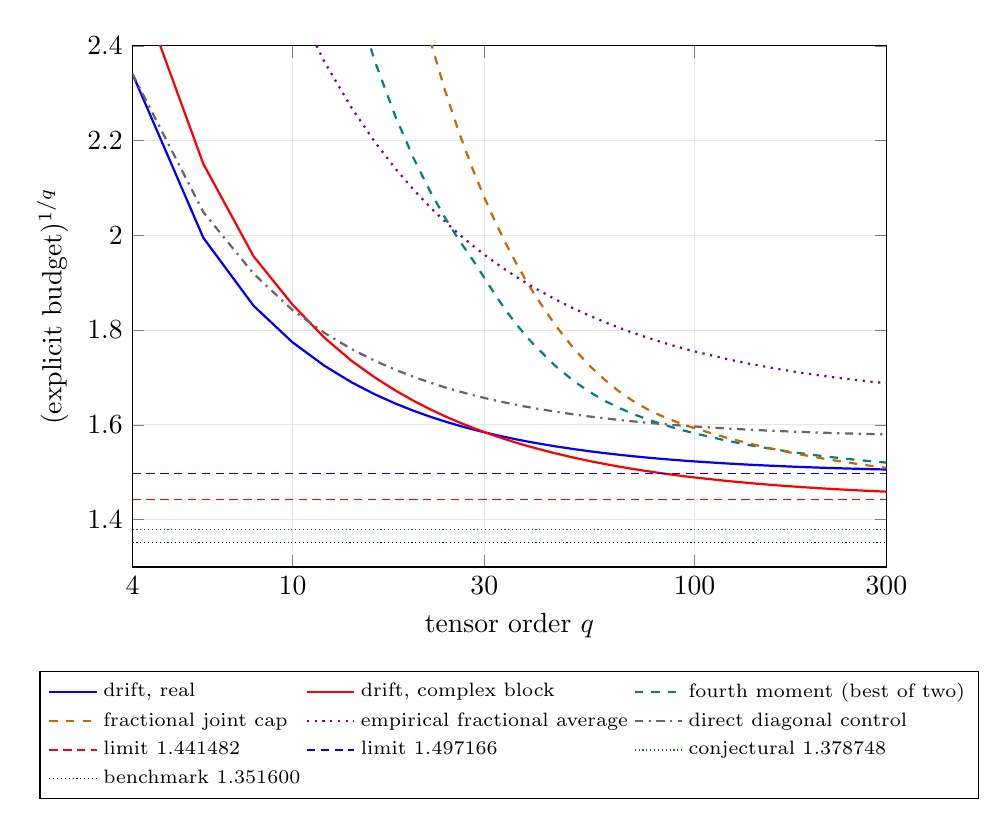
\begin{tikzpicture}
\begin{axis}[width=0.92\linewidth,height=8.2cm,xmode=log,
  xmin=4,xmax=300,ymin=1.3,ymax=2.4,
  xtick={4,10,30,100,300},xticklabels={4,10,30,100,300},
  xlabel={tensor order $q$},ylabel={(explicit budget)$^{1/q}$},
  legend style={font=\scriptsize,at={(0.5,-0.2)},anchor=north,cells={anchor=west}},
  legend columns=3,
  every axis plot/.append style={thick},restrict y to domain=1.2:2.6,
  grid=major,grid style={gray!20}]
\addplot[blue,solid] coordinates {(4,2.34035)(6,1.99476)(8,1.85133)(10,1.77417)(12,1.72476)(14,1.69006)(16,1.66457)(18,1.64509)(20,1.62967)(22,1.61714)(24,1.60679)(26,1.59807)(28,1.59065)(30,1.58424)(32,1.57865)(34,1.57374)(36,1.56938)(38,1.56549)(40,1.56201)(45,1.55466)(50,1.54882)(55,1.54405)(60,1.54009)(65,1.53674)(70,1.53388)(75,1.5314)(80,1.52924)(85,1.52734)(90,1.52564)(95,1.52413)(100,1.52277)(120,1.51847)(140,1.51541)(160,1.51312)(180,1.51134)(200,1.50991)(220,1.50875)(240,1.50778)(260,1.50696)(280,1.50626)(300,1.50565)};
\addlegendentry{drift, real}
\addplot[red,solid] coordinates {(4,2.56075)(6,2.15083)(8,1.9557)(10,1.85367)(12,1.78396)(14,1.73557)(16,1.7003)(18,1.6728)(20,1.65078)(22,1.63277)(24,1.61776)(26,1.60505)(28,1.59413)(30,1.58464)(32,1.57632)(34,1.56895)(36,1.56239)(38,1.55649)(40,1.55118)(45,1.5399)(50,1.53082)(55,1.52333)(60,1.51706)(65,1.51172)(70,1.50711)(75,1.5031)(80,1.49957)(85,1.49644)(90,1.49365)(95,1.49114)(100,1.48887)(120,1.4816)(140,1.47634)(160,1.47235)(180,1.4692)(200,1.46666)(220,1.46457)(240,1.4628)(260,1.4613)(280,1.46001)(300,1.45888)};
\addlegendentry{drift, complex block}
\addplot[teal,dashed] coordinates {(4,9.29673)(6,5.06285)(8,3.73637)(10,3.1138)(12,2.75758)(14,2.52842)(16,2.36918)(18,2.25234)(20,2.16306)(22,2.09269)(24,2.03584)(26,1.98897)(28,1.9497)(30,1.91045)(32,1.87303)(34,1.84079)(36,1.81287)(38,1.78862)(40,1.76752)(45,1.7247)(50,1.6928)(55,1.66868)(60,1.6501)(65,1.63548)(70,1.62369)(75,1.61395)(80,1.60572)(85,1.59863)(90,1.59243)(95,1.58695)(100,1.58205)(120,1.56664)(140,1.55566)(160,1.54741)(180,1.54099)(200,1.53584)(220,1.53161)(240,1.52808)(260,1.52509)(280,1.52251)(300,1.52028)};
\addlegendentry{fourth moment (best of two)}
\addplot[orange!80!black,dashed] coordinates {(4,23.68128)(6,9.59997)(8,6.04759)(10,4.56007)(12,3.76718)(14,3.28111)(16,2.95487)(18,2.72163)(20,2.54695)(22,2.41142)(24,2.30329)(26,2.21506)(28,2.14173)(30,2.07983)(32,2.02691)(34,1.98115)(36,1.94122)(38,1.90607)(40,1.87493)(45,1.81083)(50,1.76156)(55,1.72336)(60,1.69394)(65,1.67014)(70,1.65137)(75,1.63649)(80,1.6245)(85,1.61465)(90,1.60632)(95,1.59913)(100,1.59278)(120,1.57292)(140,1.55855)(160,1.54753)(180,1.53877)(200,1.53162)(220,1.52565)(240,1.52059)(260,1.51624)(280,1.51244)(300,1.5091)};
\addlegendentry{fractional joint cap}
\addplot[violet,dotted] coordinates {(4,3.87298)(6,3.07171)(8,2.71081)(10,2.50288)(12,2.36665)(14,2.2701)(16,2.19782)(18,2.14154)(20,2.09639)(22,2.05931)(24,2.02826)(26,2.00187)(28,1.97913)(30,1.95931)(32,1.94189)(34,1.92643)(36,1.91263)(38,1.90021)(40,1.88898)(45,1.86507)(50,1.84573)(55,1.82973)(60,1.81626)(65,1.80476)(70,1.7948)(75,1.7861)(80,1.77843)(85,1.77161)(90,1.7655)(95,1.75999)(100,1.75501)(120,1.73898)(140,1.72728)(160,1.71834)(180,1.71127)(200,1.70553)(220,1.70078)(240,1.69676)(260,1.69333)(280,1.69036)(300,1.68776)};
\addlegendentry{empirical fractional average}
\addplot[black!60,dashdotted] coordinates {(4,2.34035)(6,2.04898)(8,1.91912)(10,1.84213)(12,1.79408)(14,1.76026)(16,1.73545)(18,1.71638)(20,1.70129)(22,1.68904)(24,1.67891)(26,1.67038)(28,1.6631)(30,1.65682)(32,1.65135)(34,1.64653)(36,1.64226)(38,1.63845)(40,1.63503)(45,1.62783)(50,1.62209)(55,1.61741)(60,1.61352)(65,1.61024)(70,1.60743)(75,1.605)(80,1.60287)(85,1.601)(90,1.59934)(95,1.59785)(100,1.59652)(120,1.59229)(140,1.58929)(160,1.58703)(180,1.58528)(200,1.58388)(220,1.58274)(240,1.58179)(260,1.58098)(280,1.58029)(300,1.57969)};
\addlegendentry{direct diagonal control}
\addplot[red,thin,densely dashed,domain=4:300,samples=2] {1.441482};
\addlegendentry{limit $1.441482$}
\addplot[blue,thin,densely dashed,domain=4:300,samples=2] {1.497166};
\addlegendentry{limit $1.497166$}
\addplot[green!50!black,thin,densely dotted,domain=4:300,samples=2] {1.378748};
\addlegendentry{conjectural $1.378748$}
\addplot[black,thin,densely dotted,domain=4:300,samples=2] {1.351600};
\addlegendentry{benchmark $1.351600$}
\end{axis}
\end{tikzpicture}
\caption{Effective upper bases $(\text{explicit uncapped budget})^{1/q}$ against $q$ at
$n=2$, $\eps=(9/10)^q$, computed from the exact integer budgets (drift branches,
the fourth-moment and joint-cap benchmarks defined above, the empirical
fractional average and direct diagonal control of \cite{Holden}). Horizontal
lines: the limiting drift bases, the conjectural base under
Conjecture~\ref{conj:gamma}, and the analysis benchmark. The joint-cap curve
exceeds its base $1.441482$ by a factor of at least $e^{0.31/\sqrt q}$
(Proposition~\ref{prop:overhead}), so it approaches the base only slowly.}
\label{fig:bases}
\end{figure}

\paragraph{Complementary guarantees.}
The drift estimator does not dominate every earlier bound. At fixed $\eps$,
Holden's empirical fractional branch
$(q+1)\inf_{1<p\le2}\lceil(6c_n(p)^q/\eps^p)^{1/(p-1)}\rceil$ has base $2/\sqrt e=1.2131$
at $n=2$, better than $(4/\sqrt e)^{1/3}=1.3437$ (complex drift) and $e^{1/3}=1.3956$
(real drift); at $\eps=(9/10)^q$ its base is $1.6461$ (attained at $p=2$). The
combined sufficient upper bound is therefore
\[
 \min\{N,\ \text{empirical fractional},\ \mathcal D_1,\ \mathcal D_{q+1}\};
\]
the earlier Nystr\"om benchmark budgets are dominated by
Theorem~\ref{thm:domination}. Direct diagonal control remains an additional
available bound, especially when low-rank approximation is inconvenient.

%======================================================================
\section{The sharp exponent}\label{sec:sharp}
%======================================================================
Theorem~\ref{thm:drift} is sufficient, not sharp. We now show that the
per-factor exponent of the optimal drift constant is pinned between an explicit
Chernoff rate and $D_n$, and that the two-column block does not change the
lower end.

\begin{definition}
For the real one-column law or the complex block law on $(\R^n)^{\otimes q}$ let
\[
 \kappa_\opt(n,q)=\sup_{R\succeq0,\,R\ne0}\frac{\tr(R^2)/\tr R}{\E(\tr R-\tr R')},
\]
the smallest constant for which \eqref{eq:main-drift} holds. Define
\[
 \gamma_n=-\min_{0\le\lambda\le1}\log c_n(\lambda)
\]
with $c_n=c_n^{\R}$ or $c_n^{\C}$ matching the law.
\end{definition}

Here $c_n(\lambda)=\E X^\lambda$ for $X=n|w_1|^2$, $w$ uniform on the unit sphere,
so $e^{-q\gamma_n}=\min_\lambda\E\prod_jX_j^\lambda$ is the Chernoff bound for the event
$\{\prod_jX_j\ge1\}$ that a probe sees a coordinate spike at unit scale.
Convexity of $\log c_n$ with $\log c_n(0)=\log c_n(1)=0$ gives $0<\gamma_n$, and
the tangent at $1$ gives $\log c_n(\lambda)\ge-D_n(1-\lambda)$, so $\gamma_n<D_n$.
For $n=2$ complex, $\log c_2(\lambda)=\lambda\log2-\log(1+\lambda)$ is minimized at
$\lambda^*=1/\log2-1=0.4427$, giving the closed form
\[
 \gamma_2^{\C}=\log2-1-\log\log2=0.0596601 .
\]
Numerically $\gamma_2^{\R}=0.109117$, $\gamma_3^{\C}=0.080129$, $\gamma_4^{\C}=0.090435$.
Here $X=\prod_jX_j$ with $X_j\sim\mathrm{Uniform}[0,2]$ in the complex binary case.

\begin{theorem}[Sharp-exponent bracket]\label{thm:bracket}
For $n\ge2$ and $n^q\ge4$, for both the real one-column law and the complex block law,
\[
 \tfrac1{32}e^{q\gamma_n}\le\kappa_\opt(n,q)\le e^{qD_n}.
\]
Hence $\gamma_n\le\liminf_q\frac1q\log\kappa_\opt\le\limsup_q\frac1q\log\kappa_\opt\le D_n$; for
$n=2$ complex the optimal per-factor exponent lies in $[0.0597,0.1931]$, and for
$n=2$ real in $[0.1091,0.3069]$.
\end{theorem}

\begin{proof}
The upper bound is Theorem~\ref{thm:drift}. We prove the lower bound
by constructing a residual with one spike and a flat background.

\emph{Step 1: the residual and its overlap variable.}
Set
\[
 N=n^q,\qquad
 \delta=\frac1{N-1},\qquad
 u=e_1^{\otimes q},\qquad
 R=\delta I+(1-\delta)uu^{\mathsf T}.
\]
Its eigenvalues are \(1,\delta,\ldots,\delta\), so
\[
 \tr R=2,\qquad
 \tr R^2=1+\frac1{N-1},\qquad
 \frac{\tr R^2}{\tr R}\ge\frac12.
\]
Write
\[
 X=|u^*z|^2=\prod_{j=1}^q X_j,
 \qquad X_j=|x_{j,1}|^2.
\]
For \(0\le\lambda\le1\), independence gives
\(\E X^\lambda=c_n(\lambda)^q\).
Since \(\min\{X,1\}\le X^\lambda\),
\begin{equation}\label{eq:chernoff}
 \E\min\{X,1\}\le e^{-q\gamma_n}.
\end{equation}
We will also use
\[
 \frac2{N-1}\le\frac4N\le4e^{-q\gamma_n},
\]
which follows from \(\gamma_n\le D_n\le\log n\).

\emph{Step 2: the real one-column law.}
Because \(\|z\|^2=N\), the drop is exactly
\[
 \mathrm{drop}
 =\frac{(1-\delta^2)X+\delta^2N}
        {(1-\delta)X+\delta N}.
\]
For \(N\ge4\), \(1-\delta\ge2/3\) and \(\delta N\ge1\).
Hence the denominator is at least \((1-\delta)(1+X)\).
Using \(X/(1+X)\le\min\{X,1\}\) and
\(\delta^2N\le2/(N-1)\), we obtain
\[
 \E\,\mathrm{drop}
 \le\frac32\left(e^{-q\gamma_n}+\frac2{N-1}\right)
 \le8e^{-q\gamma_n}.
\]
The defining ratio for \(\kappa_\opt\) is thus at least
\(e^{q\gamma_n}/16\), which is stronger than required.

\emph{Step 3: the complex two-column block.}
Let
\[
 W=[a\ b],\quad a=\Re z,\quad b=\Im z,\quad
 G=W^{\mathsf T}W,\quad y=W^{\mathsf T}u.
\]
Here \(\|y\|^2=X\). Let \(P\) be the range projector of \(R^{1/2}W\).
Since \(R^{1/2}u=u\), the projector formula gives
\begin{align*}
 \mathrm{drop}
 &=\delta\rank P+(1-\delta)\|Pu\|^2,\\
 \|Pu\|^2
 &=y^{\mathsf T}
   \bigl(\delta G+(1-\delta)yy^{\mathsf T}\bigr)^\dagger y.
\end{align*}
The eigenvalues of \(G\) are
\[
 \frac{N\pm|z^{\mathsf T}z|}{2}.
\]
To bound the smaller one, normalize \(x_j=\sqrt n\,w_j\) and put
\[
 \Pi=\prod_{j=1}^q|w_j^{\mathsf T}w_j|,
 \qquad |z^{\mathsf T}z|=N\Pi.
\]
Independent coordinate phases imply
\[
 \E|w^{\mathsf T}w|^2
 =\sum_{a=1}^n\E|w_a|^4=\frac2{n+1}.
\]
Markov's inequality and independence therefore give
\[
 \Prob\{\Pi\ge1/2\}
 \le4\left(\frac2{n+1}\right)^q
 \le4e^{-q\gamma_n}.
\]
For the last comparison, \(\gamma_n<D_n<\log((n+1)/2)\):
check \(n=2\) directly, and use
\(D_n^{\C}<1-\gamma<\log2\) for \(n\ge3\).

On the event \(\{\Pi<1/2\}\), \(G\succeq(N/4)I\).
Define \(\sigma=y^{\mathsf T}G^{-1}y/\delta\).
Sherman--Morrison gives
\[
 \|Pu\|^2=\frac{\sigma}{1+(1-\delta)\sigma},
 \qquad
 \sigma\le\frac{4X}{\delta N}\le4X.
\]
It follows that, on this event,
\[
 \mathrm{drop}
 \le2\delta+\min\{(1-\delta)\sigma,1\}
 \le2\delta+4\min\{X,1\}.
\]
On its complement, use the deterministic bound
\(\mathrm{drop}\le\tr R=2\).
Combining these estimates with \eqref{eq:chernoff},
\[
 \E\,\mathrm{drop}
 \le\frac2{N-1}+4e^{-q\gamma_n}+8e^{-q\gamma_n}
 \le16e^{-q\gamma_n}.
\]
The numerator in the defining ratio is at least \(1/2\), so
\(\kappa_\opt\ge e^{q\gamma_n}/32\).
\end{proof}

\begin{remark}[What the block buys on the hard family]
The proof suggests a bounded-factor advantage for the two-column block:
when the real and imaginary parts have squared norms near \(N/2\),
the scalar quotient is approximately \(X/(X+L)\), whereas the block
drop is approximately \(X/(X+L/2)\), with \(L=\delta(N-1)\).
Section~\ref{sec:numerics} records a reproducible finite-order check.
The proven lower exponent applies to the two-column block; it does not
establish an exponent for the larger retained interpolation span.
\end{remark}

\begin{conjecture}\label{conj:gamma}
For the complex block law at $n=2$,
$\kappa_\opt(2,q)=e^{q\gamma_2+o(q)}$; more generally
$\frac1q\log\kappa_\opt(n,q)\to\gamma_n$ for both laws.
\end{conjecture}

If Conjecture~\ref{conj:gamma} holds, Theorem~\ref{thm:queries} with
$\kappa=e^{q\gamma_2+o(q)}$ gives the binary running base
$(2e^{\gamma_2}\cdot100/81)^{1/3}=1.378748$ (real branch: $1.401666$), an
exponential improvement of the upper record. Formally inserting $\kappa=e^{o(q)}$ into the present sufficient-bound
calculation gives $(200/81)^{1/3}=1.351600$. This is a benchmark of an analysis
that pays $N\norm{R_m}_F^2/s^2$ with
$\norm{R_m}_F^2\lesssim T^2/m$; it is not a lower bound on every algorithm
using Nystr\"om and diagonal control. The spike family suggests a possible route: the drift is controlled by the probability that a probe has
non-negligible overlap with the dominant direction, for which $\gamma_n$ gives the Chernoff upper bound used here.
Proving a matching rate for every PSD residual requires an additional argument.

%======================================================================
\section{Other probe laws}\label{sec:otherlaws}
%======================================================================
Lemma~\ref{lem:ratio} used only isotropy and a directional moment bound, and
Lemma~\ref{lem:block} only that the drop dominates a quotient. We record three
instances. The last two concern ordinary matrix--vector sketches: SRHT rows and
CountSketch vectors are not rank-one tensor queries.

\subsection{Independent sub-Gaussian factors}
\begin{proposition}\label{prop:subgauss}
Let the factors $x_j\in\R^{n_j}$ be independent and isotropic (coordinates within
a factor need not be independent, and discrete laws are allowed), with
$\E\exp(\langle x_j,u\rangle^2/K_j^2)\le2$ for all unit $u$. Then
$\E\langle x_j,u\rangle^4\le2K_j^2(K_j^2-1)$, and Theorems~\ref{thm:drift}--\ref{thm:op}
and the real branch of Theorem~\ref{thm:queries} hold with
\[
 \kappa_{\rm SG}=\prod_j2K_j^2(K_j^2-1).
\]
\end{proposition}
\begin{proof}
With $X=\langle x_j,u\rangle^2$, $e^y\ge1+y+y^2/2$ gives
$1+1/K^2+\E X^2/(2K^4)\le2$, i.e.\ $\E X^2\le2K^2(K^2-1)$. Tensorize by
Lemma~\ref{lem:moments} at $p=2$ and apply Lemma~\ref{lem:ratio} with $\beta=1$;
Lemma~\ref{lem:slope} is not needed. Zero responses obey the $0/0$ convention.
\end{proof}
Expected PSD progress needs no ordinary Gram inverse, which may fail to exist
with positive probability for such laws. For specific laws the near-one limit
$\lim_\beta\prod_jm_j(1+\beta)^{1/\beta}$ is smaller.

\subsection{A fresh SRHT row}
Let $F$ be an $n\times n$ orthogonal matrix with flat entries
$|F_{ja}|=n^{-1/2}$ (e.g.\ a normalized Walsh--Hadamard matrix), $D=\diag(\epsilon)$
with independent Rademacher signs, and $B$ any orthogonal matrix independent of
$D$ (deterministic, or itself a random sign-transform layer). A \emph{fresh row
probe} is $z=\sqrt n\,B^{\mathsf T}DF^{\mathsf T}e_J$ for a row index $J$, redrawn
independently for every probe. This covers the one-layer SRHT ($B=I$) and the
two-layer transform $FDF'D'$.

\begin{imported}[Sharp Khintchine inequality {\cite{Haagerup}}]\label{imp:khintchine}
For $r\ge2$, real $a$ and Rademacher $\epsilon$,
$\E|\sum_ia_i\epsilon_i|^r\le\E|g|^r\norm a^r$, $g\sim N(0,1)$.
\end{imported}

\begin{proposition}\label{prop:srht}
A fresh row probe is isotropic and $\E|u^{\mathsf T}z|^{2p}\le g(p)\norm u^{2p}$ with
$g(p)=2^p\Gamma(p+1/2)/\sqrt\pi$ for $p\ge1$. Consequently
Theorems~\ref{thm:drift}--\ref{thm:op} hold for independent fresh rows with
\[
 \kappa_0=\lim_{\beta\downarrow0}g(1+\beta)^{1/\beta}=e^{\log2+\psi(3/2)}=\frac{e^{2-\gamma}}2=2.0743278 .
\]
This is the dimension-uniform bound obtained by the same moment argument for
i.i.d.\ Rademacher or Gaussian probes in $\R^N$, and the $n\to\infty$ limit of
$e^{D_n^{\R}}$. It need not be the best constant at a fixed finite dimension.
\end{proposition}
\begin{proof}
$u^{\mathsf T}z=\sum_a\epsilon_a(\sqrt nF_{Ja})(Bu)_a$ is a Rademacher sum with
coefficient norm $\norm{Bu}=\norm u$; apply Imported Theorem~\ref{imp:khintchine}
with $r=2p$ conditionally on $B$. Isotropy: $\E zz^{\mathsf T}=nB^{\mathsf T}\diag(F_{J\cdot}^2)B=I$.
Since $g(1)=1$, $\kappa_0=\exp\{(\log g)'(1)\}=\exp\{\log2+\psi(3/2)\}$ and
$\psi(3/2)=2-\gamma-2\log2$. For i.i.d.\ Rademacher probes the directional
moments are bounded by the same $g(p)$; flat directions approach Gaussian
moments as the dimension grows. Thus the dimension-uniform bounds coincide; and $D_n^{\R}=\log n+\psi(3/2)-\psi(n/2+1)\to\log2+\psi(3/2)$.
\end{proof}
Thus the same dimension-uniform sufficient drift constant applies to a
fresh SRHT row and to an unstructured Rademacher probe. This comparison of
upper bounds does not establish equality of their optimal drift constants. The rows of one SRHT sketch share $D$; after one row is
used the residual is correlated with the others, so the $M$ rows of a single
sketch are \emph{not} $M$ independent updates, and this proposition does not
count them as such.

\subsection{Whole CountSketch blocks}
Let $H\in\R^{b\times N}$ be a CountSketch block: independent uniform hashes
$h_i\in[b]$ and independent signs $\sigma_i$, $H_{h_i,i}=\sigma_i$. The update is
$R'=R-RH^{\mathsf T}(HRH^{\mathsf T})^\dagger HR$.

\begin{lemma}[Mixed trace identity]\label{lem:cs}
For symmetric $B,R$ and $X_B=\tr(HBH^{\mathsf T})$,
$\E X_B=\tr B$ and
\[
\begin{aligned}
 \E(X_BX_R)
 &=\tr B\tr R+\frac2b\left(\tr(BR)-\sum_iB_{ii}R_{ii}\right)\\
 &\le\left(1+\frac2b\right)\tr B\tr R
 \qquad(B,R\succeq0).
\end{aligned}
\]
\end{lemma}
\begin{proof}
$X_B=\tr B+\sum_{i\ne j}B_{ij}\sigma_i\sigma_j\mathbf1_{h_i=h_j}$. In the product of two
such sums only matching unordered pairs survive the sign expectation, each with
hash probability $1/b$, giving $(2/b)\sum_{i\ne j}B_{ij}R_{ij}$. For PSD matrices
$\tr(BR)\le\tr B\tr R$ and $B_{ii}R_{ii}\ge0$.
\end{proof}

\begin{theorem}[CountSketch block drift]\label{thm:cs}
With $\kappa_b=1+2/b$, for every nonzero PSD $R$ and every finite convex
$f\ge0$ with $f(0)=0$,
\[
 \E(\tr R-\tr R')\ge\frac{\tr R^2}{\kappa_b\tr R},\qquad
 \E\tr f(R')\le\tr f(R)-\frac{\tr[Rf(R)]}{\kappa_b\tr R}.
\]
Hence Theorems~\ref{thm:relative}--\ref{thm:op} hold for $s$ independent blocks
with $\kappa_b$ in place of $\kappa$ and $s$ counting blocks.
\end{theorem}
\begin{proof}
Let $F=R^{1/2}H^{\mathsf T}HR^{1/2}$ and $P$ its range projector. Each eigenvalue of
$F$ is at most $\tr F=X_R$, so $F\preceq X_RP$ and
$\tr(PR)\ge\tr(FR)/X_R=X_{R^2}/X_R$, and likewise $\tr(Pf(R))\ge X_{Rf(R)}/X_R$.
Under $dQ=X_B\,dP/\tr B$, Jensen gives
$\E[X_B/X_R]\ge(\tr B)^2/\E(X_BX_R)\ge\tr B/(\kappa_b\tr R)$ (Lemma~\ref{lem:cs};
$X_R=0$ forces $X_B=0$ when $\ker R\subseteq\ker B$). The compression argument
of Theorem~\ref{thm:convex} finishes the proof.
\end{proof}

\begin{remark}[Scope: one block is credited like one probe]
The bound uses $F\preceq(\tr F)P$ and so credits a $b$-column block with the
progress of a single normalized probe. For rank-one residuals it is within $\kappa_b$ of the maximal possible drop.
Already for $R=I_N$ with $N\gg b$, it loses a factor of order $b$: the true drop
is the number of nonempty buckets, about $b$, while the bound gives
$1/\kappa_b$. In sketch-column count these guarantees are therefore
weaker than per-column bounds by up to a factor $b$; their merits are the
explicit constant and the use of independence only across blocks.
\end{remark}

%======================================================================
\section{Reproducible numerical checks}\label{sec:numerics}
The accompanying
\href{https://github.com/DiarHaidary/Results/blob/main/manuscripts/02-Product-Probe-Drift/verify_numerics.py}{verification script}
and
\href{https://github.com/DiarHaidary/Results/blob/main/manuscripts/02-Product-Probe-Drift/verification_results.json}{machine-readable results}
recompute the constants and budgets in double precision.
They also run a seeded Monte Carlo experiment and check selected matrix
identities. These checks support the calculations; they do not replace
the proofs.

\subsection{Constants and integer budgets}
The two binary order-one constants are
\[
 e^{D_2^{\R}}=1.3591409142,\qquad
 e^{D_2^{\C}}=1.2130613194.
\]
A central finite difference for \((\log c_n)'(1)\), for both fields and
\(n\in\{2,3,5,10\}\), agrees with \(D_n\) within \(1.1\cdot10^{-10}\).
Numerical minimization over \([0,1]\) gives
\[
 \gamma_2^{\R}=0.1091170039,\qquad
 \gamma_2^{\C}=0.0596601011.
\]
The latter agrees with the closed form in Section~\ref{sec:sharp}.
The leading comparison ratios are \(18.441745\) and \(44.230199\).

Table~\ref{tab:budgets} uses \(n=2\), \(\eps=(9/10)^q\).
All counts are uncapped; the algorithm may instead use \(N=2^q\) calls.
The script evaluates the displayed integer formulas. For large ranges
of the auxiliary rank, it searches around the continuous minimizer;
the table is a numerical optimization check, not an independent
certificate of the global integer optimum.

\begin{table}[ht]
\centering
\begin{tabular}{@{}rrrr@{}}
\toprule
\(q\) & real drift & complex drift & direct diagonal control\\
\midrule
8 & 138 & 214 & 184\\
12 & 693 & 1,039 & 1,112\\
16 & 3,474 & 4,880 & 6,770\\
20 & 17,457 & 22,583 & 41,264\\
24 & 87,699 & 103,261 & 251,564\\
30 & 987,645 & 995,187 & 3,786,870\\
40 & 55,885,335 & 42,312,585 & 347,540,288\\
\bottomrule
\end{tabular}

\medskip
\begin{tabular}{@{}rrrr@{}}
\toprule
\(q\) & fourth-moment benchmark & fractional benchmark & empirical fractional\\
\midrule
8 & 37,984 & 1,789,197 & 2,916\\
12 & 193,348 & 8,169,539 & 30,875\\
16 & 985,320 & 33,776,624 & 296,395\\
20 & 5,027,762 & 131,952,535 & 2,688,105\\
24 & 25,694,427 & 497,015,252 & 23,495,275\\
30 & 271,702,808 & 3,474,278,491 & 579,594,817\\
40 & 7,844,091,534 & 83,059,865,691 & 111,965,394,931\\
\bottomrule
\end{tabular}
\caption{Explicit uncapped query budgets. The two panels separate the new
drift construction from the comparison formulas.}
\label{tab:budgets}
\end{table}
The exact drift integers switch from the real branch to the complex branch
at \(q=31\), both for \(\eps=(9/10)^q\) and for \(\eps=0.1\), in the checked
range \(2\le q\le60\). This agrees with the leading-term crossover of
Proposition~\ref{prop:crossover}.

\subsection{The spike-plus-flat family}
We draw \(20{,}000\) independent complex-spherical product probes for each
tensor order, using the random seed \(20260929\). The input is the family
in the proof of Theorem~\ref{thm:bracket}, with \(n=2\).
Table~\ref{tab:spike} reports the expected drop divided by
\(\tr R^2/\tr R\); parentheses give one estimated standard error.
The experiment uses exact two-by-two formulas for the block Gram matrix
and does not expand the ambient tensor.

\begin{table}[ht]
\centering
\begin{tabular}{@{}rcccc@{}}
\toprule
\(q\) & scalar quotient & two-column block & \(1/\kappa_{\C}\) & \(e^{-q\gamma_2}\)\\
\midrule
4 & 0.713 (0.003) & 1.077 (0.004) & 0.462 & 0.788\\
6 & 0.581 (0.004) & 0.808 (0.004) & 0.314 & 0.699\\
8 & 0.483 (0.004) & 0.650 (0.004) & 0.213 & 0.620\\
10 & 0.404 (0.004) & 0.541 (0.004) & 0.145 & 0.551\\
12 & 0.337 (0.004) & 0.451 (0.004) & 0.098 & 0.489\\
14 & 0.283 (0.003) & 0.380 (0.004) & 0.067 & 0.434\\
\bottomrule
\end{tabular}
\caption{Seeded spike-family experiment. The Chernoff column is a rate
benchmark, not a claimed lower bound on the expected drop.}
\label{tab:spike}
\end{table}
The observed block/quotient ratios range from approximately \(1.33\)
to \(1.51\). Each observed progress value exceeds the proved sufficient
bound \(1/\kappa_{\C}\). This finite-order experiment neither establishes
the conjectured asymptotic exponent nor evaluates the larger retained
interpolation span.

\subsection{Algebraic spot checks}
For PSD matrices of dimensions \(4,8,12\), including singular inputs,
the sequential-update identity in Lemma~\ref{lem:sequential} agrees with
a direct pseudoinverse calculation to Frobenius error below
\(9\cdot10^{-15}\). The numerical construction includes rank-one,
intermediate-rank, and full-rank matrices. These small checks are
diagnostics of the implementation, not a proof of the identity.

%======================================================================
\section{Open problems}\label{sec:open}
%======================================================================
\begin{enumerate}
\item \textbf{Close the exponent bracket.} Prove Conjecture~\ref{conj:gamma}:
a drift constant $e^{q\gamma_n+o(q)}$ for the complex block (or the real probe).
At $n=2$, $\eps=(9/10)^q$ this lowers the upper base from $1.441482$ to
$1.378748$. A natural route is a mixed-moment argument that keeps the event
$\{|u^*z|^2\gtrsim1\}$ rather than the average log-moment.
\item \textbf{Improve the analysis benchmark.} The present variance and
Frobenius bounds give base $1.351600$ if one formally removes the exponential
drift penalty. This is a sufficient-bound benchmark, not an algorithmic
impossibility result. Better residual-specific diagonal bounds, or adaptive
pivoting after a probe, could improve it.
\item \textbf{Block-level mixed moments.} Replace $\tr F$ by $\lambda_{\max}(F)$ in
the CountSketch and complex-block arguments to credit a block with more than one
probe's progress.
\item \textbf{Retention.} Quantify the gain of the retained $(q+1)$-span; the
numerics suggest a constant factor only, which should be proved.
\item \textbf{Stability and bits.} Numerically stable interpolation nodes and a
polynomial-size discretization of the angular laws (Appendix~\ref{app:finite}
is existential).
\item \textbf{Relative spectral error.} A rank-$r$ relative operator-norm
analogue of Theorem~\ref{thm:op} for product probes, without OSE-level sketch sizes.
\end{enumerate}

\appendix
%======================================================================
\section{Finite randomness with arbitrarily small slack}\label{app:finite}
%======================================================================
\begin{lemma}[Finite isotropic angular laws]\label{lem:finite}
Fix $n$, $p>1$ and $\delta>0$. There is a finite law of nonzero rational raw
vectors over $\R$, or Gaussian-rational raw vectors over $\C$, with dyadic
probabilities, whose formal normalization $x=\sqrt n\,g/\norm g$ satisfies
$\E xx^*=I$ and $\sup_{\norm u=1}\E|u^*x|^{2p}\le c_n(p)+\delta$.
\end{lemma}
\begin{proof}
Approximate a standard Gaussian scalar by symmetric finite laws on nonzero
rational half-grid points with dyadic probabilities, converging weakly. Use
i.i.d.\ coordinates (two copies per coordinate in the complex case). Coordinate
permutations and sign changes (and multiplication by $i$ in the complex case)
are symmetries, so the normalized covariance is scalar with trace $n$: exact
isotropy. Normalization is continuous away from $0$, where the Gaussian has no
atom, so the angular laws converge weakly to the uniform sphere law. The
functions $x\mapsto|u^*x|^{2p}$, $\norm u=1$, are bounded and equicontinuous on
the compact sphere; a finite net in $u$ gives uniform convergence of their
expectations.
\end{proof}
This follows the angular construction of \cite[Section~6]{Holden}.

\begin{proposition}[Finite-law drift]\label{prop:finite}
For every $\eta>0$ the finite laws can be chosen so that all drift-based bounds
hold with $(1+\eta)\kappa$.
\end{proposition}
\begin{proof}
Choose $\beta>0$ with $H(1+\beta)^{1/\beta}<(1+\eta)\kappa$ and then local tolerances
$\delta_j$ with $[\prod_j(c_{n_j}(1+\beta)+\delta_j)]^{1/\beta}\le(1+\eta)\kappa$.
Tensorization and isotropy hold for the finite laws, and Lemma~\ref{lem:ratio}
at this $\beta$ gives drift with $(1+\eta)\kappa$. At a zero denominator the
numerator vanishes. The algorithm queries raw rational factors; normalization
rescales a real column or a whole complex block by one positive scalar,
preserving the Nystr\"om output. Interpolation uses rational nodes; the other
batches use fair signs and the bounded-bit coordinate law.
\end{proof}
This preserves the quantitative guarantees, not almost-sure rank recovery.

%======================================================================
\begin{thebibliography}{99}
\bibitem{MSW}
R.~A. Meyer, W.~Swartworth, and D.~P. Woodruff,
\emph{Understanding the Kronecker matrix-vector complexity of linear algebra},
Proc.\ 42nd ICML, PMLR 267 (2025), 43909--43933; \href{https://arxiv.org/abs/2502.08029v2}{arXiv:2502.08029v2}.

\bibitem{MA}
R.~A. Meyer and H.~Avron,
\emph{Hutchinson's estimator is bad at Kronecker-trace-estimation},
SIAM J.\ Matrix Anal.\ Appl.\ 47 (2026), 353--387; \href{https://arxiv.org/abs/2309.04952v2}{arXiv:2309.04952v2}.

\bibitem{RA11cat}
OpenProblemsInNLA catalogue,
\emph{RA-11: Optimal trace-estimation complexity using Kronecker matrix-vector queries},
\href{https://github.com/ajt60gaibb/OpenProblemsInNLA/blob/main/randomized-and-low-rank-approximation/RA-11/README.md}{Problem statement}, accessed 29 September 2026.

\bibitem{Holden}
S.~Holden,
\emph{RA-11: probability-sensitive product probes and diagonal correction},
public working paper, 14 September 2026; Corollary~2.3 and Sections~4--7.
\href{https://github.com/ajt60gaibb/OpenProblemsInNLA/blob/main/references/holden-further-2026-09-14/RA-11/manuscript.md}{Public proof text}.
The interpolation simulation is Lemma~4.2.

\bibitem{CETW}
Y.~Chen, E.~N. Epperly, J.~A. Tropp, and R.~J. Webber,
\emph{Randomly pivoted Cholesky: practical approximation of a kernel matrix with
few entry evaluations}, Comm.\ Pure Appl.\ Math.\ 78 (2025), 995--1041; \href{https://arxiv.org/abs/2207.06503}{arXiv:2207.06503}.

\bibitem{Epperly}
E.~N.~W. Epperly,
\emph{A new analysis of the randomly pivoted Cholesky algorithm},
\href{https://arxiv.org/html/2608.20633v1}{arXiv:2608.20633v1} (2026), Lemma~4.2.

\bibitem{DG}
R.~Divan and M.~A. Gilles,
\emph{Convergence rates of randomly pivoted methods for low-rank approximation},
\href{https://arxiv.org/html/2609.06287v1}{arXiv:2609.06287v1} (2026).

\bibitem{CEMT}
C.~Cama\~no, E.~N. Epperly, R.~A. Meyer, and J.~A. Tropp,
\emph{Faster linear algebra algorithms with structured random matrices},
\href{https://arxiv.org/abs/2508.21189v1}{arXiv:2508.21189v1} (2025).

\bibitem{SVB}
A.~K. Saibaba, B.~D. Verma, and G.~Ballard,
\emph{Improved analysis of Khatri--Rao random projections and applications},
\href{https://arxiv.org/abs/2507.23207v2}{arXiv:2507.23207v2} (2026).

\bibitem{BM}
L.~Beretta and C.~Musco,
\emph{A tight analysis of Khatri--Rao oblivious subspace embeddings},
\href{https://arxiv.org/abs/2608.28094v3}{arXiv:2608.28094v3} (2026).

\bibitem{FTU}
Z.~Frangella, J.~A. Tropp, and M.~Udell,
\emph{Randomized Nystr\"om preconditioning},
SIAM J.\ Matrix Anal.\ Appl.\ 44 (2023); \href{https://arxiv.org/abs/2110.02820v2}{arXiv:2110.02820v2}.

\bibitem{Haagerup}
U.~Haagerup,
\emph{The best constants in the Khintchine inequality},
Studia Math.\ 70 (1981), 231--283. \href{https://doi.org/10.4064/sm-70-3-231-283}{doi:10.4064/sm-70-3-231-283}.
\end{thebibliography}
\end{document}
